\section{Log}
\label{appendix_log}

\subsection{Week 1 - 02/02/24}
\label{log:week1}

Task: Our task was to make the \texttt{minitwit.py} run with python v3
instead of python v2.

Steps taken:

\begin{enumerate}
    \item We copied the source code from the server
\end{enumerate}

\begin{minted}{bash}
    scp -r student@164.90.160.52:/home/student/itu-minitwit ~/Desktop/
\end{minted}

\begin{enumerate}
    \item We also copied the database which was saved as a \texttt{*.db} file with
\end{enumerate}

\begin{minted}{bash}
    $ scp student@164.90.160.52:/tmp/minitwit.db \textasciitilde{}/Desktop/itu{-}minitwit
\end{minted}

\begin{enumerate}
    \setcounter{enumi}{2}
    \item Then we created a Github organization with a repository called itu-minitwit
    \item We clone the minitwit repo
\end{enumerate}

\begin{minted}{bash}
    $ git clone https://github.com/devops2024-group-e/itu-minitwit.git
\end{minted}

\begin{enumerate}
    \def\labelenumi{\arabic{enumi}.}
    \setcounter{enumi}{4}
    \item We copied the files from \texttt{\textasciitilde{}/Desktop} to the location where we cloned the repo
    \item We tried to run the application by using the \texttt{control.sh} script. But got an error message that it were missing the database. We saw that the database file actually should be located in the \texttt{/tmp} and not in the current working directory of the application. So we placed the database in \texttt{/tmp} and then it worked.
    \item We then started doing the steps to convert the application from python 2 to python 3. First we used the \texttt{2to3} tool to convert to see what has to be changed.
\end{enumerate}

\begin{itemize}
    \item We changed the reading of the database file to read it as \texttt{UTF-8}
    \item Added parenthesis to the print statement
    \item In the tests we changed the assertions to use \texttt{rv.text} instead of \texttt{rv.data} as the \texttt{rv.data} is in a binary format and that we are trying to look for a particular string.
\end{itemize}

\begin{enumerate}
\setcounter{enumi}{7}
    \item After that we ran the \texttt{shellcheck} on \texttt{control.sh}. Here we added the shebang (\texttt{\#!/bin/bash}) to the top of the file.
    \item After all of this we tried to look into the difference between \texttt{python} and \texttt{python3} command \href{https://stackoverflow.com/questions/64801225/python-or-python3-what-is-the-difference}{(take a look here)}. After looking into it we decided to just use the \texttt{python3} command in order to make sure that the tools we use actually runs python3.
\end{enumerate}

\subsection{Week 2 - 09/02/24}
\label{log:week2}

Task: Our task was to refactor minitwit to C\# and RazorPages.

Steps taken:

\subsubsection{Refactorization:}
\label{log:refactorization}

\textbf{index.cshtml:}

\begin{itemize}
    \item Made @page \{tl : string\} optional
\end{itemize}

\textbf{index.cshtml.cs:}

\begin{itemize}
    \item Added a string path
\end{itemize}

\textbf{index.cshtml:}

\begin{itemize}
    \item Display tweets
    \item for loop for all messages
\end{itemize}

\textbf{index.cshtml.cs:}

\begin{itemize}
    \item Created public list for messages
    \item We copied the original .css file and added in the new .css
    \item Checking if there is messages and printing them
    \item We tried to install codegenerator - it didn't work. Line of command:
    \item We created login.cshtml and linked it to page and model LoginModel
\end{itemize}

\textbf{Layout:}

\begin{enumerate}
    \item We created the `Shared' folder under `Pages' to hold UI that we wish to use across different pages. Here we then added \texttt{\_Layout.cshtml} and rewrote the code in \texttt{layout.html} from the python source code to match the correct format of `.cshtml' files to encompass the same UI format.
    \item We added the \texttt{style.css} file from the original project and  added it to the `wwwroot' folder under the name \texttt{main.css}.  This was done to connect the html and css properly, so that the refactored version of the website now matched the original one in terms of looks.
\end{enumerate}

\textbf{Login:}

\begin{enumerate}
    \item Created a \texttt{Login.cshtml} that contains the same logic as in the python version by adding pieces of the page one at a time.
    \item Added an in memory user (let us call it a dummy user) as we do not have the database connected for now and we just want to see if the UI logic actually works when a user tries to login
    \item Adding a session that should store the \texttt{userid} as it does in the python application. We do this by adding the following lines as settings in the \texttt{Program.cs}:

    \begin{minted}{csharp}
        builder.Services.AddDistributedMemoryCache();

        builder.Services.AddSession(options =>
        {
            options.IdleTimeout = TimeSpan.FromMinutes(5);
            options.Cookie.HttpOnly = true;
            options.Cookie.IsEssential = true;
        });


        app.UseSession();
    \end{minted}
    \item Now we can get and set session data by using \texttt{this.HttpContext.Session.SetString()} and \texttt{this.HttpContext.Session.GetString()} in a \texttt{PageModel} class
    \item Add if statement that if the login is successful then it should store \texttt{userid} and redirect to \texttt{/Timeline} (Timeline should take care if it should show a public or user timeline)
\end{enumerate}

\textbf{Register:}

\begin{enumerate}
    \item Created the \texttt{Register.cshtml} and added the same UI logic that is present in the corresponding python template \texttt{register.html}
    \item Then the \texttt{Register.cshtml.cs} page model that handles the request to the site was created, with the model that is necessary in order to register
    \item We tested the site if it worked as it should but figured that the page model did not capture what was typed because we missed the \texttt{BindProperty} on the properties in the page model. So we added that
    \item After, we had to adjust the validation if statement to work correctly due to a missing negation of the \texttt{Email.Contain("@")}
\end{enumerate}

\textbf{Timeline:}

\begin{itemize}
    \item Trying to add switches between the different timelines. Trying to make it show different titles based on user.

    \begin{itemize}
        \item I cannot make it work by ``just'' adding another if/else in time index.cs file.
        \item I don't where the title ``Public'' on public timeline gets set as it says ``Public Timeline'' in the switch in index.cs file.
        \item Turns out the connections we had made before relied on getting the path and doing some operations on that, but that is the wrong way to get the path. You just get the path as input to the \texttt{OnGet} method, and from there I make a simple switch and send it on to the html.
        \item A lot of help came from: \url{https://www.learnrazorpages.com/}

        \begin{itemize}
            \item \url{https://www.learnrazorpages.com/razor-pages/routing}
            \item \url{https://www.learnrazorpages.com/razor-pages/forms}
        \end{itemize}
    \end{itemize}

    \item Added a bit of different views for logged-in user, other-user and public timeline.
    \item Added shared view for submitting a message.
    \item A lot of functionality still depends of having a database where users and messages are stored

    \begin{itemize}
        \item Knowing whether we have a logged-in user
        \item Knowing the connection between users (following/not following)
        \item Having the messages stored in a database and store more messages as times goes on
    \end{itemize}
\end{itemize}

\subsubsection{Connecting to a
database:}
\label{log:connecting-to-a-database}

\begin{enumerate}
    \item In \href{http://Setup.sh}{Setup.sh} we added the dotnet ef tool version 7.0.1
    \item Added designpacket ****\texttt{dotnet\ add\ package\ {[}Microsoft.EntityFrameworkCore.Design{]}(http://Microsoft.EntityFrameworkCore.Design)\ —version\ 7.0.1}
    \item Added sqllite package to the project \texttt{dotnet\ add\ package\ {[}Microsoft.EntityFrameworkCore.{]}(http://Microsoft.EntityFrameworkCore.Design)Sqlite—version\ 7.0.1}
    \item Referenced database, \texttt{dotnet\ ef\ dbcontext\ scaffold\ “Datasource=/temp/minitwit.db”\ Microsoft.EntityFrameworkCore.Sqlite\ -o\ Models\ —context-dir\ .}
    \item Scaffold wants us to provide a connection string (first argument) and which sql provider we use (second argument)
    \item We want to place the models and context a specific place, which is specified at the end of the command
    \item Injected dependencies - adding services to container
\end{enumerate}

\subsubsection{Issues with creating
endpoints}
\label{log:issues-with-creating-endpoints}

Since we tried to use the ``pure'' razor template we had some trouble trying to create the exact same endpoints that was present in the \texttt{{[}minitwit.py{]}(http://minitwit.py)} and \texttt{minitwit\_tests.py}. We tried to create our own custom routing via:

\begin{minted}{csharp}
    services.AddRazorPagesOptions(options => {
        options.Conventions.AddPageRoute("<Ref to page>", "new/route/to/page");
    });
\end{minted}

However, the above solution to our endpoint path problems couldn't mitigate the issue. For that reason we looked at what we could do in order to solve our issue. And in the official documentation we found another way to create Razor pages with the MVC architecture. So we decided to pivot and create an MVC project. Luckily we could copy the contents of both \texttt{*.cshtml} pages and \texttt{*.cshtml.cs} files from one project to another.

\subsection{Week 3 - 16/02/24}
\label{log:week3}

Task: Our task was to create a simulation API and deploy the program

Steps taken:

\subsubsection{Setting up a basic VM in Digital Ocean using Vagrant}
\label{log:setting-up-a-basic-vm-in-digital-ocean-using-vagrant}

\begin{enumerate}
    \item We installed Vagrant on our machines (mac: \texttt{brew\ install\ -\/-cask\ vagrant} )
    \item Followed this guide in order to generate keypairs \url{https://www.digitalocean.com/community/tutorials/how-to-set-up-ssh-keys-on-ubuntu-1804}
    \item Registered public key on digital ocean and received a digital ocean token.
    \item We set two environment variables in ``which file?''
    \item We run this command \texttt{\$\ vagrant\ plugin\ install\ vagrant-digitalocean}
    \item We then run \texttt{vagrant\ up} with the exercise files and got it to work
    \item We made sure to destroy the dbserver and webserver.
    \item We then made a new branch in our project and copied the vagrantfile in the exercises session to our own project.
    \item We renamed dbserver and webserver to dbserver\_new and webserver\_new in order to being able to differ them from the exercise servers (important that we destroyed the right ones)
    \item We noticed that the IP address for the dbserver that was needed in order to get the webserver didn't work now
    \item We then figured out that we had to name them with dash instead in order for the names to work with the vagrantfile, now we renamed them to dbserver-new and webserver-new
    \item We started making the vagrantfile more personalized to our program and included what we need. Like dotnet, sqlite etc.
\end{enumerate}

\subsubsection{Setting up a simulation API}
\label{log:setting-up-a-simulation-api}

\begin{enumerate}
    \item We followed this tutorial: \url{https://learn.microsoft.com/en-us/aspnet/core/tutorials/first-web-api?view=aspnetcore-7.0\&tabs=visual-studio-code} up until the point about the controller being scaffolded. There we deviated and used the same bash script that we used for the original system. This helped us set up an API skeleton with connected Swagger for us to have a starting point to work with.
    \item We copied over the \emph{Controllers}, \emph{Models} and \emph{ViewModels} folders in order to have the same logic as the original refactored Minitwit system.
    \item We rewrote the different controllers to then fit the logic of the python API simulator given by Helge. This mostly entailed returning the specified status codes instead of redirecting to certain pages, since the API isn't concerned with the view of the system.

    \begin{enumerate}
        \item We checked that the controllers worked as expected by inspecting swagger and testing the HTTP requests with different input to see if the methods behaved accordingly.
    \end{enumerate}
    \item After finishing writing the API, we added a folder \emph{Test}, which contains Helge's python API simulator \texttt{{[}minitwit\_sim\_api.py{]}(https://github.com/itu-devops/lecture\_notes/blob/master/sessions/session\_03/API\_Spec/minitwit\_sim\_api.py)}, and ran it against our API. The same folder contains guides on how to run these programs against each other.

    \begin{itemize}
        \item Here we encountered consistently error codes in the form of 400's and 500's. After troubleshooting and inspecting the files given by Helge, we figured out that our minitwit project were using the session ID in order to check whether or not a user was logged in. This clashed with the API tests which were checking whether the ``Authorization'' part of the HTTP header was equal to a certain code. We then rewrote the login function for our API along with the functions affected by no longer being able to pull information from the session ID.
    \end{itemize}

    \item After rewriting the API, all test but 1 from Helge's API simulator passed and the work was added to that weeks release.
\end{enumerate}

\begin{center}\rule{0.5\linewidth}{0.5pt}\end{center}

Possible issues if recreating:

\begin{enumerate}
    \item Note that when running the \texttt{scaffold-db.sh}, it may transform the model classes to use \texttt{byte{[}{]}} types instead of the original \texttt{string}.
\end{enumerate}

\subsubsection{Managing the database through the dotnet App}
\label{log:managing-the-database-through-the-dotnet-app}

In the process of refactoring from python to C\#, we still had some
minor things that needed to be moved when we look specifically at the
database. These things are:

\begin{itemize}
    \item Create the database (This removes the last dependency to flask in the \texttt{{[}minitwit.py{]}(http://minitwit.py)} app)
    \item Get the connectionstring to the database from the configuration
    \item Add Composite Primary Key to Follwers table such that the Entity Framework can track changes to it
\end{itemize}

We did the changes by in the following order:

\begin{enumerate}
    \item First we looked at the website in order to see how we can create the db. We figured that it was possible to do it with \texttt{dotnet\ ef\ database\ update} at the respective project where the Entity Framework \texttt{MinitwitContext.cs} file is.
    \item We then the command line \texttt{dotnet\ ef\ database\ update} to the \texttt{{[}control.sh{]}(http://control.sh)} file. But i ran into an issue that i changed the working directory.

    \begin{enumerate}
        \item This was fixed by looking into how to change the working directory and executing a particular command at that location.
    \end{enumerate}
    \item Then we changed the \texttt{Makefile} at init to use the \texttt{{[}control.sh{]}(http://control.sh)\ init}.
    \item Now that we can create the database with dotnet, we removed the \texttt{{[}minitwit.py{]}(http://minitwit.py)}
    \item After that we looked into how we can get the connectionstring from configuration. We found out that .NET Framework has created some different providers that we can use. Since there already was two settings files, namely \texttt{appsettings.json} and \texttt{appsettings.Development.json} we decided to use them, and incorporate the possibility to override them using the Environment Variables with a \texttt{Minitwit\_*} prefix. So we included this in the \texttt{program.cs}.
    \begin{minted}{csharp}
        // Register source of configurations
        builder.Configuration
            .AddJsonFile("appsettings.json", optional: false, reloadOnChange: true)
            .AddJsonFile($"appsettings.{builder.Environment.EnvironmentName}.json", optional: true)
            .AddEnvironmentVariables(prefix: "Minitwit_");
    \end{minted}
    \item Then we added the connection-string in the settings files.
    \item And included the connection-string at startup of Entity Framework in the application with

    \begin{minted}{csharp}
        builder.Services.AddDbContext<MinitwitContext>(options =>
        {
            options.UseSqlite(builder.Configuration.GetConnectionString("MinitwitDatabase"));
        });
    \end{minted}
    \item Last but not least. To finish the changes with the database we changed the database schema to have a composite primary key. Usually this would be a good idea to do in a SQL Schema. But since the database is being initialized by EntityFramework, then this description was changed in the \texttt{MinitwitContext.cs} file. To be more specific we added a line with \texttt{HasKey(e\ =\textgreater{}\ new\ \{\ e.WhoId,\ e.WhomId\ \});} to the Follower entity.
    \item But this change has to be reflected on the \texttt{Follower.cs} model as well. So we had to remove the possibility that the \texttt{WhoId} and \texttt{WhomId} could be \texttt{null}
\end{enumerate}

\subsection{Week 4 - 23/02/24}
\label{log:week4}

Task: Finish creating an API for the simulator to call. Setup CI/CD.
Deploy Minitwit

Steps taken:

\subsubsection{API:}
\label{log:api}

\begin{enumerate}
    \item We realized that the API was missing an endpoint \texttt{/latest.} We wrote a separate controller to handle this functionality, where it finds the largest command ID under the table `Latest' in the database and returns it.
    \item We also missed that every HTTP request called a method called \texttt{UpdateLatest} as the first order of business. We rewrote this function to C\# where it adds the current command ID to the data base under the table `Latest'.
\end{enumerate}

\subsubsection{CI/CD:}
\label{log:cicd}

\begin{enumerate}
    \item We copy Helge's example yaml file and work from this, by renaming and restructuring to fit our own setup.
    \item We stumble upon the cache-to and cache-from options but fail to understand what these actually do and how it works. We decide to delete them from our yaml file for now, but return later or ask for help.

    \begin{itemize}
        \item By looking around online, we stumbled across this link: \url{https://docs.docker.com/build/cache/backends/gha/} where it seemed that it wasn't necessary to manually insert the URL and token, since it is given earlier in the file. So we kept the formatting as seen in the link, which also was present in Helge's original file
    \end{itemize}
    \item Because we have our images in the GitHub container repository, we changed the login from docker hub to ghcr(github container registry)

    \begin{itemize}
        \item The docker images were moved to here in order to keep information such as password to the servers private
        \item We used this link: \url{https://github.com/docker/login-action} and modified what was written under ``Service account based authentication'' to fit to ghcr
    \end{itemize}
    \item We removed the part about testing, since we currently don't have a docker image for testing our code. This should be worked in at a later date.
\end{enumerate}

Task: Ensure that the backend (API), the frontend, and the database are
running on the server

Steps taken:

\subsubsection{Vagrant}
\label{log:vagrant}

\begin{enumerate}
    \item We realised that the \texttt{Vagrantfile} set up last week, was in large part not usable for the purposes that we needed, since all we really needed was to set up the server and accessing it, we rewrote the \texttt{Vagrantfile}.
    \item We wrote a guide on how to create and access the server using vagrant: \href{https://www.notion.so/Connecting-to-the-Digital-Ocean-server-using-vagrant-5b8564d3a0fd40bdbc2c326705f1f8dc?pvs=21}{Connecting to the Digital Ocean server using vagrant}
    \item Later this approach was changed by adding the following to the \texttt{.ssh/config} file.

    \begin{minted}{bash}
        host devops
            Hostname 161.35.78.128
            User root
            Identityfile ~/.ssh/do_ssh_key
    \end{minted}
    Which meant the server could be reached by simply typing \texttt{ssh\ devops}.
\end{enumerate}

\subsubsection{Docker}
\label{log:docker}

\begin{enumerate}
    \item We created dockerfiles and docker hub repositories for the frontend, the backend, and the database.
    \item We built these images locally and then pushed them to pinkvinus repo on dockerhub.
    \item However, we realised that we didn't like to have the images publicly available to we created our docker images with \texttt{ghcr.io/devops2024-group-e/\textless{}image\ name\textgreater{}:\textless{}version\ tag\textgreater{}}. We need the first part of the docker image name tag because it references to the registry where it should push and later get the docker image from. So an example of a command in the shell we used is:
    \begin{minted}{bash}
        docker build -f Dockerfile.backend . -t ghcr.io/devops2024-group-e/backend.minitwit:latest
    \end{minted}
    \item The way we published the images to see if it worked was with the following commands in order:
\begin{minted}{bash}
    docker build -f Dockerfile.backend . -t ghcr.io/devops2024-group-e/backend.minitwit:latest
    docker build -f Dockerfile.frontend . -t ghcr.io/devops2024-group-e/frontend.minitwit:latest
    docker build -f Dockerfile.database . -t ghcr.io/devops2024-group-e/db.minitwit:latest

    # Authenticate to the github private container registry
    docker login ghcr.io -u <github username> -p <github token>

    # Push the build images to the container registry
    docker push ghcr.io/devops2024-group-e/backend.minitwit:latest
    docker push ghcr.io/devops2024-group-e/frontend.minitwit:latest
    docker push ghcr.io/devops2024-group-e/db.minitwit:latest
\end{minted}
    \item We ran the docker images locally first and it worked perfectly. We could connect to the database and everything. We tested this by performing:

\begin{minted}{bash}
    docker run -p 5432:5432 --name database -d ghcr.io/devops2024-group-e/db.minitwit:latest
    docker run -p 80:80 --name frontend -d ghcr.io/devops2024-group-e/frontend.minitwit:latest
    docker run -p 8080:8080 --name backend -d ghcr.io/devops2024-group-e/backend.minitwit:latest
\end{minted}
    And then we tried to poke around in the website to see if it actually   had access to the database. We also used the \texttt{minitwit\_test.py} to test that the site still worked accordingly.
    \item Now we add a \texttt{remote-server} directory that contains the scripts that deploys and setups the server. In there we create \texttt{{[}init.sh{]}(http://init.sh)} which create the docker containers when the server is being created and we create \texttt{{[}deploy.sh{]}(http://deploy.sh)} which is used when a new image of backend and frontend has been created.
    \item We then used vagrant up to see if it worked. It created the server\ldots{} but. It cannot create and use the containers based on the docker images we have created because it has been built by the platform \texttt{linux/arm64} but the server needs \texttt{linux/amd64}.

    \begin{enumerate}
        \item To resolve this we have looked at using the ---platform flag. This did not solve it. Actually we had a hard time trying to build the images on Mac
        \item We then built the images from the workflow and this made it work
    \end{enumerate}
    \item On the server, we removed the created containers that could not run and ran \texttt{{[}init.sh{]}(http://init.sh)} in the \texttt{/minitwit} directory. And it almost worked. It could not connect to the database.

    \begin{enumerate}
    \item No matter what if we change the connectionstring to use \texttt{Host=localhost} or \texttt{Host=127.0.0.1} with port \texttt{5432} it does not work.
    \item We decided to create a docker compose file and express the network. Here we can reference the name of the database container in the connectionstring in the \texttt{Host} part of the connectionstring.

        \begin{enumerate}
            \item IT WORKED!!!
        \end{enumerate}
    \end{enumerate}
    \item We create the docker compose file in the \texttt{remote-server} directory such that when we provision the server then it is included.

    \begin{enumerate}
        \item Also modifying the \texttt{{[}deploy.sh{]}(http://deploy.sh)} script to:

\begin{minted}{bash}
    echo $DOCKER_PASSWORD | docker login ghcr.io -u $DOCKER_USERNAME --password-stdin
    docker run --platform linux/amd64 -p 80:80 -d ghcr.io/devops2024-group-e/frontend.minitwit
    docker run --platform linux/amd64 -p 8080:8080 -d ghcr.io/devops2024-group-e/backend.minitwit
\end{minted}
    \end{enumerate}
\end{enumerate}

\subsection{Week 5 - 01/03/24}
\label{log:week5}

Task: Clean repository. Abstract database. Include testing in our
workflow.

Steps taken:

\subsubsection{Clean repository:}
\label{log:clean-repository}

\subsubsection{Abstract database:}
\label{log:abstract-database}

\begin{itemize}
    \item In order to abstract the database layer, we have created repository classes in a separate Infrastructure project which can be called from the application and the API. We have also added tests for these in a separate test project. The benefit of this is that we don't write SQL directly in the methods, but instead we abstract them out such that they can be reused.
\end{itemize}

\begin{enumerate}
    \item Added Repository + Repository interface
    \item Replaced calls to \texttt{MinitwitContext} with calls to the individual repositories (with dependency injection)
    \item Made sure in \texttt{Program.cs} that the correct repositories are given in the dependency injection when building
    \item Wrote tests for the repositories with mock database

    \begin{itemize}
        \item \texttt{dotnet\ add\ package\ Microsoft.EntityFrameworkCore.InMemory\ -\/-version\ 7.0.2} package added to be able to test the database abstraction on an in-memory mock database.
    \end{itemize}
\end{enumerate}

\subsubsection{Add testing to workflow:}
\label{log:add-testing-to-workflow}

We started by creating a ``skeleton'' workflow that would only run when a pull request was opened, which consisted of setting up both python and Dotnet along with their needed dependencies to then test that the correct versions had been chosen.

We then removed the python since we only used it to test if the workflow worked as expected. We then set up the database and ran the frontend in order to run the endpoint tests, which was the test setup we at that time could incorporate into the workflow.

Test for other parts of the system will be added at a later stage, when they are available.

We then played around with the best option for which types of pull requests should trigger this workflow. After several tries, we ended up with having no restrictions on the type, as being too specific caused the workflow not to be activated when it needed to be. This means that closing a PR and opening it again reruns the workflow whether it passed or not the first time and likewise for other situations. This ensured that we always tested the new code before merging it into main.

\subsubsection{Fix last step of workflow: deploy step}
\label{log:fix-last-step-of-workflow-deploy-step}

The workflow prints the following in the deploy step:
\begin{minted}{bash}
    Error: Cannot perform an interactive login from a non TTY device
    no configuration file provided: not found
    no configuration file provided: not found
    no configuration file provided: not found
\end{minted}

\begin{enumerate}
    \item Found that the issue could be related to not providing credentials to the \texttt{—password-stdin} flag of \texttt{docker\ login.}
    \item Create \texttt{{[}test.sh{]}(http://test.sh)} script on the server with the original \texttt{docker\ login} line of the script and set file permission with \texttt{chmod\ +x\ /minitwit/test.sh}. Ran \texttt{ssh\ \textless{}user\textgreater{}@\textless{}server\textgreater{}\ -i\ \textless{}ssh\ key\textgreater{}\ -o\ StrictHostKeyChecking=no\ \textquotesingle{}/minitwit/test.sh\textquotesingle{}} and can confirm that same output
    \item Verified that the \texttt{DOCKER\_USERNAME} and \texttt{DOCKER\_PASSWORD} was on the server
    \item Change the login line to be \texttt{docker\ login\ ghcr.io\ -u\ "\$\{DOCKER\_USERNAME\}"\ -p\ "\$\{DOCKER\_PASSWORD\}"}
    \item Tried the test script again. Now it works.
    \item Remove \texttt{{[}test.sh{]}(http://test.sh)} on the server
    \item Add the new \texttt{docker\ login} line in \texttt{{[}init.sh{]}(http://init.sh)} and \texttt{{[}deploy.sh{]}(http://deploy.sh)} script in our repo
    \item After PR approval and merge, add script changes to the server manually
\end{enumerate}

\subsection{Week 6 - 08/03/24}
\label{log:week6}

Tasks: Add monitoring. Fix unresolved issues from last week. Refine
logging.

Steps taken:

\subsubsection{Beginning Migrate Database}
\label{log:beginning-migrate-database}

\begin{enumerate}
    \item Since we do not have a configuration management tool yet we decided to create the database as a managed service. We need to setup Ansible so that we have an automated way to setup the database in the future. An issue is created.
    \item In the DigitalOcean UI we only allowed private services to connect and Andreas public IP
    \item Now we are installing PGAdmin so that we can connect.
    \item In order to connect to database securely we do the following:

    \begin{enumerate}
        \item Go into DigitalOcean
        \item Navigate to the database resource
        \item Download CA certificate
        \begin{enumerate}
            \item Install certificate in system
        \end{enumerate}

        \item Take login parameters and insert into connection details in PGAdmin when adding a connection(Use the public connection not PVC)
    \end{enumerate}
    \item Create minitwit database
    \item Create minitwit-web user
    \item Execute \texttt{schema.sql} on minitwit database
    \item Create role and add permissions to select, delete, update, and insert records in the public schema on minitwit database

    \begin{minted}{sql}
        CREATE ROLE minitwit_app_executer;
        GRANT SELECT, UPDATE, INSERT, DELETE ON ALL TABLES IN SCHEMA public TO minitwit_app_executer;
    \end{minted}
    \item We(or I, Andreas) got tired and decided to not perform the migration until we have more time\ldots{}
\end{enumerate}

\subsubsection{Add monitoring:}
\label{log:add-monitoring}

\begin{enumerate}
    \item We first added a new configuration similar to our minitwit configuration in our vagrant file
    \item Move our \texttt{remote-server} directory into an \texttt{.infrastructure} directory and changed the synced folder in our vagrant file
    \item Change the synced directory on our \texttt{minitwit-monitor} vagrant config
    \item Add a docker compose file containing the grafana application and expose on port 80
    \item Login with admin and changed password
    \item Change the docker compose file to run prometheus
    \begin{enumerate}
        \item Add \texttt{prometheus.yml} in order to add applications and be ready to get metrics
    \end{enumerate}

    \item Add docker \texttt{daemon.json} file in \texttt{/etc/docker} in order to expose docker metrics for prometheus

    \begin{enumerate}
        \item Restart docker on app server in order to expose metrics
    \end{enumerate}
\end{enumerate}

\subsubsection{Add monitoring code to backend:}
\label{log:add-monitoring-code-to-backend}

Added:

\begin{minted}{bash}
    dotnet add package OpenTelemetry.Exporter.Prometheus.AspNetCore --version 1.4.0-rc.4
    dotnet add package OpenTelemetry.Extensions.Hosting
    dotnet add package OpenTelemetry.Instrumentation.AspNetCore
\end{minted}

Added to Program.cs:

\begin{minted}{csharp}
    builder.Services.AddOpenTelemetry()
    .WithMetrics(b => b.AddPrometheusExporter());

    app.UseOpenTelemetryPrometheusScrapingEndpoint();
\end{minted}

\subsubsection{Add monitoring code to frontend:}
\label{log:add-monitoring-code-to-frontend}

Adding monitoring to the frontend entailed the exact same steps as
adding monitoring to the backend. The following code got added to:

\textbf{Minitwit.csproj}

\begin{minted}{xml}
    <PackageReference Include="OpenTelemetry.Exporter.Prometheus.AspNetCore" Version="1.7.0-rc.1" />
    <PackageReference Include="OpenTelemetry.Extensions.Hosting" Version="1.7.0" />
    <PackageReference Include="OpenTelemetry.Instrumentation.AspNetCore" Version="1.7.1" />
\end{minted}

\textbf{Program.cs}

\begin{minted}{csharp}
    builder.Services.AddOpenTelemetry()
        .WithMetrics(b => b.AddAspNetCoreInstrumentation()
                            .AddPrometheusExporter());

    app.UseOpenTelemetryPrometheusScrapingEndpoint();
\end{minted}

\subsubsection{Fix unresolved issues from last week:}
\label{log:fix-unresolved-issues-from-last-week}

\subsubsection{Fix implementation of database abstraction layer so integration tests does not fail:}
\label{log:fix-implementation-of-database-abstraction-layer-so-integration-tests-does-not-fail}

Integrations tests are failing for the implementations. Might be because
the sql statements should be changes to another sql language.

\subsubsection{Fix integrations tests:}
\label{log:fix-integrations-tests}

\subsubsection{Fix testing workflow visualisation in github actions:}
\label{log:fix-testing-workflow-visualisation-in-github-actions}

\subsubsection{Refine logging:}
\label{log:refine-logging}

This task was downprioritized during the week, but these initial links
for inspiration has been found.

\url{https://learn.microsoft.com/en-us/aspnet/core/fundamentals/logging/?view=aspnetcore-7.0\#log-level}
\url{https://learn.microsoft.com/en-us/aspnet/core/fundamentals/logging/?view=aspnetcore-7.0\#log-category}
\url{https://stackify.com/csharp-logging-best-practices/}

\subsection{Week 7 - 15/03/24}
\label{log:week7}

Tasks: Add logging. Provide feedback for group f.~Add configurations
management.

Steps taken:

\subsubsection{Provide feedback for group f:}
\label{log:provide-feedback-for-group-f}

\begin{itemize}
    \item Do you see a public timeline? Yes
    \item Does the public timeline show messages that the application received from the simulator? Hmm. I see messages on the public timeline, but all the dates are from 2009 and i figure that if they were created by the simulator, the dates would be newer?
    \item Can you create a new user? Yes
    \item Can you login as a new user? Yes
    \item Can you write a message? Yes
    \item After publishing a message, does it appear on your private timeline? Yes
    \item Can you follow another user? Yes, and afterwards i see the user's messages on my private timeline.
\end{itemize}

Very good job all in all!!

\subsubsection{Add logging:}
\label{log:add-logging}

Adding log messages to the code:

\begin{itemize}
    \item In the controllers in Minitwit and SimulatorApi statements like the one below have been added where it makes sense:
\end{itemize}


\begin{minted}{csharp}
    _logger.LogDebug($"FollowUnfollowUser returns Forbid because user is not logged in");
\end{minted}

\subsubsection{Setting up Loki and Promtail:}
\label{log:setting-up-loki-and-promtail}

We followed this youtube video: \url{https://www.youtube.com/watch?v=pnycjg_9M-o\&t=664s\&ab_channel=Thetips4you} that explained how to set up Loki and Promtail to grafana alongside this link: \url{https://ghazanfaralidevops.medium.com/grafana-loki-promtail-complete-end-to-end-project-d698aaa636d6}

\begin{itemize}
    \item The youtube video linked some already made config files for Loki and Promtail that we could use, where we then changed to the right names end urls for our system. We added the two new config files to the monitoring server and added Loki and Promtail in the \texttt{docker-compose.yaml} file.
    \item For listening on our web server, we added the Promtail config file there as well and added Promtail to the \texttt{docker-compose.yaml} file in that server as well.
    \item At first we weren't getting the correct logs written by Amalie, that we knew should be displayed. We found out that this was due to following the tutorial too closely. Instead of getting our logs from /var/log/*, we had to get them from /var/lib/docker/containers. Adding the right path was the fix to our problem and we could immediately see the correct logs appearing in Grafana.
\end{itemize}

\subsubsection{Adding configurations management:}
\label{log:adding-configurations-management}

\subsubsection{Setup an Ansible control node}
\label{log:setup-an-ansible-control-node}

\begin{itemize}
    \item Moved the vagrantfile that creates the web, and api application into the .infrastructure
    \item Made a new vagrantfile in the parentdir where the configuration management server would be set up
    \item In here we add installation commands to install the \texttt{ansible} package. This package comes with pre installed collections that contains different modules which we can later use in out ansible playbooks.
\end{itemize}

\hypertarget{make-file-to-config-management-server-called-do_ssh_key}{%
\subsubsection{Make file to config management server called
do\_ssh\_key}\label{make-file-to-config-management-server-called-do_ssh_key}}

First I added the following line to \texttt{.bashrc}

\begin{minted}{bash}
    export CONF_DO_TOKEN=<some token>
\end{minted}

Then I added the following to the

\begin{itemize}
    \item To upload the ssh key to digital ocean it needed the doctl which was first installed using snap
    \item Then the server generates a keypair without a passphrase
    \item We add the conf token to the server s.t. it knows which project we're working with
    \item Then we have to check whether DO already has a key of this name. If it does, we remove it
    \item We add the previous public key to DO
\end{itemize}

\subsubsection{Create and push Ansible playbooks}
\label{log:create-and-push-ansible-playbooks}

Our strategy is to create two initial playbooks. One for our monitoring
server and one for our web server. The documentation in Ansible and
vagrant only specifies that the vagrant file that defines our web and
monitoring server only needs to be referenced in the vagrant file as a
new provisioner. We want the provisioning script in our root vagrantfile
that creates the configuration management server to run vagrant up again
and create the other servers. Here are the steps:

\begin{itemize}
    \item Add playbook files for web and monitoring in their respective \texttt{.infrastructure} server directories.
    \item Alter the names of the servers in the Vagrant file to have test in them
    \item Create the configuration management server again
    \item Run vagrant up in the configuration management server

    \begin{itemize}
        \item It halts and waits forever when provisioning
    \end{itemize}
    \item Remove the hosts in the Ansible playbooks
    \item Run \texttt{vagrant\ up} again from the configuration management server

    \begin{itemize}
        \item Still halts and waits forever
    \end{itemize}
    \item Getting tired and frustrated at vagrant\ldots{} having a discussion with the group about vagrant the following friday
\end{itemize}

\subsection{Week 8 - 22/03/24}
\label{log:week8}

Tasks: Add three different linters. Setup Code Climate. Setup SonarQube.
Add UI testing. Add Integration testing. Add end to end testing.

Steps taken:

\subsubsection{Continuation of setting up Ansible}
\label{log:continuation-of-setting-up-ansible}

After having a talk with the other group members, we decided to not
create a solution with ansible that collaborates with Vagrant. After
some recent frustrations, we will look into which tool to use in the
future to create the infrastructure. The steps taken here is to create a
way to make ansible work in a github workflow and prepare the new
infrastructure when we have to change accounts due to money expiration
issues:

\begin{itemize}
\item By looking at the guide at github about creating a custom github action we can do it with a docker container.
\item Create a new test repo for testing provisioning of VMs using github workflows

    \begin{itemize}
        \item Include existing docker compose files and scripts for the two categories of VM's
    \end{itemize}
    \item Create a docker file for the custom github action which should contain Ansible
    \item Add a requirements file to ensure that we install specific versions of collections
    \item Build and run docker image locally with

    \begin{minted}{bash}
        docker build -t ansible:latest .
        docker run -it --rm ansible:latest bash
    \end{minted}

    \begin{itemize}
        \item Run \texttt{ansible\ -\/-version} to see that ansible is indeed installed
        \item Run \texttt{ansible-galaxy\ collection\ list} to see that the collections is installed
    \end{itemize}
    \item Create a make file for local development of the Dockerfile that contains two sections, namely build and run which performs the two commands stated above.
    \item Create github workflow to build and push the docker image to our private repo
    \item In order to create the custom github action we do the following:

    \begin{itemize}
        \item Create directory at \texttt{.github/actions/\textless{}custom-action-name\textgreater{}}
        \item Create a file called \texttt{action.yaml}
        \item Create a new dockerfile that builds on top of the docker image we have created. It only needs to create an entrypoint that executes the \texttt{{[}entrypoint.sh{]}(http://entrypoint.sh)} script
        \item Create the \texttt{{[}entrypoint.sh{]}(http://entrypoint.sh)} script which contains a call to the \texttt{ansible-playbook} command to run the playbook. The playbook will be provided as a argument defined by the action.yaml.
    \end{itemize}
    \item Create a new github workflow that uses the custom github action. We do so by referencing the path

    \begin{minted}{yaml}
        - name: Provision and deploy web servers
          uses: .github/actions/ansible-run-playbook
    \end{minted}
    \item Add parameters to the github action

    \begin{minted}{yaml}
        inputs:
            dotoken:
                description: 'The Digital Ocean token'
                required: true
            dosshkeyname:
                description: 'The name of the ssh key in Digital Ocean'
                required: true
            sshkey:
                description: 'The private ssh key to access servers'
                required: true
            dockeruser:
                description: 'The username for the docker registry'
                required: true
            dockerpassword:
                description: 'The password for the docker registry'
                required: true
            inventoryfile:
                description: 'The working directory to run the command in'
                required: true
            playbook:
                description: 'The playbook to run'
                required: true
            working-directory:
                description: 'The working directory to run the command in'
                required: true
            runs:
            using: 'docker'
            image: 'Dockerfile'
            args:
                - ${{ inputs.sshkey}}
                - ${{ inputs.dockeruser }}
                - ${{ inputs.dockerpassword }}
                - ${{ inputs.dotoken }}
                - ${{ inputs.dosshkeyname }}
                - ${{ inputs.inventoryfile }}
                - ${{ inputs.playbook }}
                - ${{ inputs.working-directory }}
    \end{minted}

    \item Add arguments in the workflow with the \texttt{with} keyword
    \item Run the workflow
    \item For the web playbook we gradually added more modules to it:

    \begin{itemize}
        \item Add firewall rules to the playbook with the \texttt{community.general.ufw} module
        \item Run the workflow
        \item Add folder synchronization with the \texttt{ansible.posix.synchronization} module for the web-playbook
        \item Run the workflow
        \item Add login and logout of docker
        \item Run the workflow\ldots{} fails

        \begin{itemize}
            \item Add arguments in the \texttt{{[}entrypoint.sh{]}(http://entrypoint.sh)} script to include docker username and docker password
        \end{itemize}

        \item Run the workflow
        \item Add \texttt{docker\_compose\_v2} module to run docker compose up
        \item Run the workflow\ldots{} fails - Could not find the module

        \begin{itemize}
            \item Ensure that the module is typed correctly - running workflow again fails
            \item Try install \texttt{ansible-core} that has no collections installed to be sure that it uses the collection installed through the \texttt{requirement.yaml} - running workflow again fails
            \item Try move the installed modules to a known directory - running workflow again still fails with cannot find the module
            \item Reference the collection in the web-playbook.yaml - running workflow again stil fails with cannot find the module:

            \begin{minted}{yaml}
                collections:
	                community.docker:<version>
            \end{minted}

            \item Rollback to use \texttt{ansible} instead of \texttt{ansible-core} and replace the docker compose module with a \texttt{shell} module and run \texttt{docker compose up\ -d}

            \begin{itemize}
                \item This works!!!!!
            \end{itemize}
        \end{itemize}
    \end{itemize}
    \item Now we copy paste the web-playbook to the monitor-playbook and change the settings to fit its state
    \item Run the playbook by adding it in the workflow - and it works!
    \item Move the github custom action related stuff to a new repo called \texttt{ansible-action}
    \item Create the new provisioning workflow in \texttt{itu-minitwit} but to not add any particular triggers since we will use it once we shift to new infrastructure

    \begin{itemize}
        \item We reference the custom github action from the repo \texttt{ansible-action} by doing multiple checkouts and reference to the path it is checked out to:

        \begin{minted}{yaml}
            - name: Login to GitHub Container Registry
              uses: docker/login-action@v3
              with:
                registry: ghcr.io
                username: ${{ secrets.DOCKER_USER }}
                password: ${{ secrets.DOCKER_PWD }}

            - name: Checkout repository
              uses: actions/checkout@v4
              with:
                path: main

            - name: Fetch Ansible Playbook action
              uses: actions/checkout@v4
              with:
                repository: devops2024-group-e/ansible-action
                sparse-checkout: |
                  .github/actions/ansible-run-playbook
                sparse-checkout-cone-mode: false
                path: action

            - name: Provision and deploy web servers
              uses: ./action/.github/actions/ansible-run-playbook
              with:
                dotoken: ${{ secrets.DIGITAL_OCEAN_TOKEN }}
                dosshkeyname: ${{ secrets.DIGITAL_OCEAN_ANSIBLE_SSH_KEY_NAME }}
                sshkey: ${{ secrets.ANSIBLE_SSH_KEY }}
                dockeruser: ${{ secrets.DOCKER_USER }}
                dockerpassword: ${{ secrets.DOCKER_PWD }}
                inventoryfile: inventory.ansible
                playbook: web-playbook.yaml
                working-directory: main/.infrastructure
        \end{minted}
    \end{itemize}
\end{itemize}

\subsubsection{Add three different linters:}
\label{log:add-three-different-linters}

Installing precommit:
\begin{minted}{bash}
    brew install pre-commit
    pre-commit sample-config > .pre-commit-config.yaml
    dotnetformaturl="https://pkgs.dev.azure.com/dnceng/public/_packaging/dotnet7/nuget/v3/index.json"
    dotnet tool install -g dotnet-format --version "7.*" --add-source $dotnetformaturl
\end{minted}

We also add the different linters to the config.yaml file.

We now want to add \texttt{hadolint}. We do so first by adding the
hadolint to the \texttt{.pre-commit-config.yaml}.

Then we try to run pre commit with \texttt{pre-commit\ run\ -a} and
could see that hadolint was not installed.

Now we install hadolint with \texttt{brew\ install\ hadolint}.

Now we add the \texttt{dotnet-format} linter to the pre commit config

We ran the pre-commit hooks but the dotnet formatter failed. So we
installed dotnet sdk 8 and ran it again. Now it works!

In order to have hooks that run automatically when we commit, we run
\texttt{install\ pre-commit}.

\subsubsection{Setup code climate:}
\label{log:setup-code-climate}

\begin{itemize}
    \item Registred to code climate and added our repository
    \item \url{https://codeclimate.com/github/devops2024-group-e/itu-minitwit}
\end{itemize}

\subsubsection{Setup SonarQube:}
\label{log:setup-sonarqube}

In order to analyze the software quality and technical debt of our project, we had to set up SonarQube as one of the tasks for the project work this week.

This was already a part of the given exercises, which meant that Helge had specified a guide in the lecture material on how to assemble it. Here he recommended the groups to use SonarCloud, which is another product from the same company behind SonarQube. The difference between the two services is that SonarCloud is a cloud-based service that easily integrates with GitHub.com, whereas SonarQube requires installation and maintenance on our server.

When registering on SonarCloud, one is able to use their GitHub login, which also makes adding the necessary repositories easier. You're then able to start add a new project by pressing the `+' button found in the top right corner and pressing `\emph{Analyze new project}', where you then have to give the application access to the specified repositories, which in our case is the minitwit repository.

Setting up your project will require you to decide on how to define what is considered new code. I here chose that this should be based on number of days, which is currently set to 30. This means that any code written in the last 30 days is considered new code. This is the recommended option for projects with continuous delivery like ours. The number of days can be changed if the current variable isn't suitable for our needs.

You are given two main options for setting up the actual analysis. You can choose methods such as GitHub Actions and other CI tools or you can choose automatic analysis if your used programming languages are supported by SonarCloud. This step wasn't specified in Helge's tutorial, so I chose to go with the automatic analysis, which was also the recommended option.

After this, the setup was complete and you can now see the measures of reliability, security and maintainability to mention a few. SonarCloud will from this point run on its own and start analyzing pull request when opened and any new code added to the main branch. The link can be found on the front page of our Notion.

\begin{center}\rule{0.5\linewidth}{0.5pt}\end{center}

After the set up was complete, I tried to figure out how to add code coverage since this wasn't added automatically. What I found out in my research was that code coverage wasn't automatically a part of the analysis when using the automatic analysis and you would have to introduce a separate third party tool, which would then send the information to SonarCloud to be analyzed. However, it does seems to be available when setting up the analysis with GitHub actions.

I discussed this with some of the members of the team and we decided to let it be for now, since the original task was just to set up SonarCloud and to instead bring it up for discussion in our next meeting to see whether we feel like code coverage in SonarCloud is a necessity in our project work.

\subsubsection{Add UI testing with Selenium:}
\label{log:add-ui-testing-with-selenium}
First we want to add Selenium to the test project along with the package for the ChromeDriver so we can do tests in Chrome browser. We also add WebDriverManager, as that seems important for getting the webdrivers to work in github actions, as well as WaitExtensions, so we can specify wait time when waiting for pageload etc.

\begin{itemize}
    \item Add Selenium to test project with following commands:

    \begin{itemize}
        \item \texttt{dotnet\ add\ package\ Selenium.WebDriver}
        \item \texttt{dotnet\ add\ package\ Selenium.WebDriver.ChromeDriver}
        \item \texttt{dotnet\ add\ package\ WebDriverManager}
        \item \texttt{dotnet\ add\ package\ Selenium.WebDriver.WaitExtensions}
    \end{itemize}
\end{itemize}
Then a folder is added to the Testing project named \texttt{UITests}, where standard testing files are added.
We have added three testing files:

\begin{itemize}
    \item \texttt{LoginRegisterLogoutUITests.cs}
    \item \texttt{FollowUnfollowUITests.cs}
    \item \texttt{MessagesUITests.cs}
\end{itemize}
All three initialise a Chrome driver and make it navigate to the localport, where the frontend is running, before executing the tests.

When the tests have been written the UI testing setup is also included in github actions by making sure to add a step in the \texttt{Frontend-Tests} in the \texttt{Testing.yml} that runs the PR-frontend, such that the tests can find the port they are testing on.

\subsubsection{Add integration testing:}
\label{log:add-integration-testing}

\subsubsection{Add end to end testing:}
\label{log:add-end-to-end-testing}

\subsubsection{Fix timestamps indatabase}
\label{log:fix-timestamps-in-database}

First we want to create a test environment such that we can try and do migrations in our own local setup. We do so by dumping the data we currently have in the database on our docker container as the following:
\begin{minted}{bash}
    pg_dump -U minitwit_sa -f dump.sql --column-inserts --data-only minitwit
\end{minted}

We could have done this in a smarter way but now we want to extract that dump file from the container:

\begin{minted}{bash}
    docker exec -it database /bin/sh -c "cat dump.sql" > dump.sql
\end{minted}

And then we want to copy that file to our local machine with the following command(executed from our local machine, which has a ssh config with a reference to our prod server called \texttt{devops}):

\begin{minted}{bash}
    scp devops:/minitwit/dump.sql ./dump.sql
\end{minted}

Now because i have to try out different things, i have created a make file with two ``commands'' namely \texttt{db-up} and \texttt{db-down}. This is to quickly refresh the database. For that reason a \texttt{db-refresh} is also created that leverages these two commands:

\begin{minted}{bash}
    .PHONY: db-down
    db-down:
        docker exec -it minitwit-dev-database /bin/sh -c "psql -U minitwit-sa minitwit -c 'TRUNCATE TABLE follower, \"user\", message, latest'"

    .PHONY: db-up
    db-up:
        docker cp ./dump.sql minitwit-dev-database:/db-setup/dump.sql
        docker exec -it minitwit-dev-database /bin/sh -c "psql -U minitwit-sa minitwit < /db-setup/dump.sql" > /dev/null

    .PHONY: db-refresh
    db-refresh: db-down db-up

\end{minted}

Now i can begin the work. First i look if we can just change the type in our table \texttt{message} from \texttt{integer} to \texttt{bigint}. We do so with the following query:

\begin{minted}{sql}
    ALTER TABLE message
	ALTER COLUMN pub_date TYPE bigint;
\end{minted}

That was allowed by the local test database without any issues. And since the datatype was a \texttt{integer} before it has converted it to a \texttt{bigint} before, because it has the same values a before.

Now I change the type in our schema file \texttt{schema.sql}. And then i change the datatype in the class \texttt{Message} to
\texttt{long}.

Now we want to display it in a beautiful format. We start by doing the following:

\begin{itemize}
    \item Create a Viewmodel for messages where the type for a timestamp is \texttt{DateTime}.
    \item Then we Convert the types we get from SQL to the viewmodel
    \item In the view we can then format the string by using \texttt{ToString("\textless{}Format\ for\ datetime\ string\textgreater{}")}
    \item We tried to use the \texttt{DisplayFormatAttribute} with \texttt{Html.For} in the view but resulted in a wrong format exception all the time. So we kept the original solution with \texttt{ToString()}.
\end{itemize}

\subsubsection{Analyse and fix the slow response time of the register endpoint}
\label{log:analyse-and-fix-the-slow-response-time-of-the-register-endpoint}

We have found that the password hash makes up the majority of the time it takes to add a new user to the system:

\begin{figure}[H]
\centering
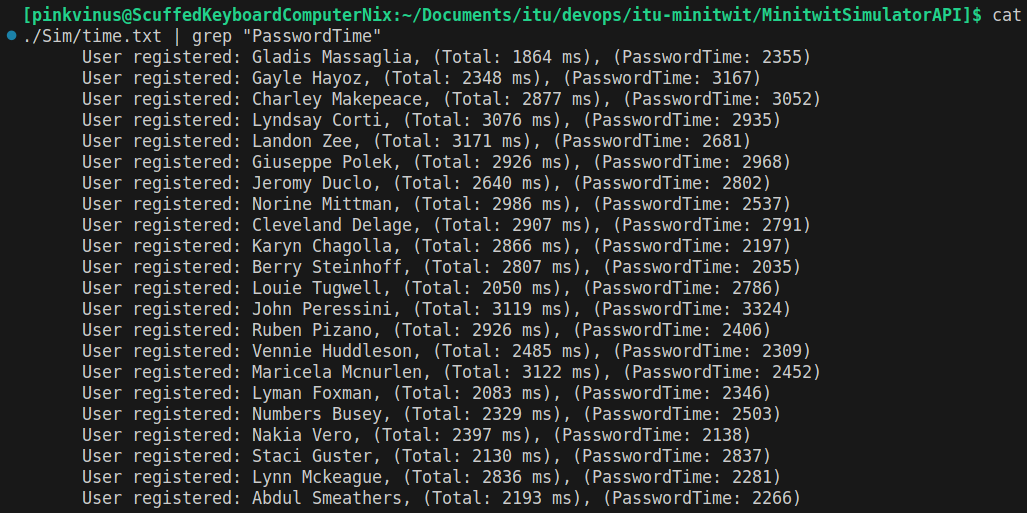
\includegraphics[width=0.7\linewidth]{password2.png}
\caption{Results from calling the register endpoint}
\end{figure}

Reducing the number of iterations (from 600000 to 6000) results in a much reduced response time

\begin{figure}[H]
\centering
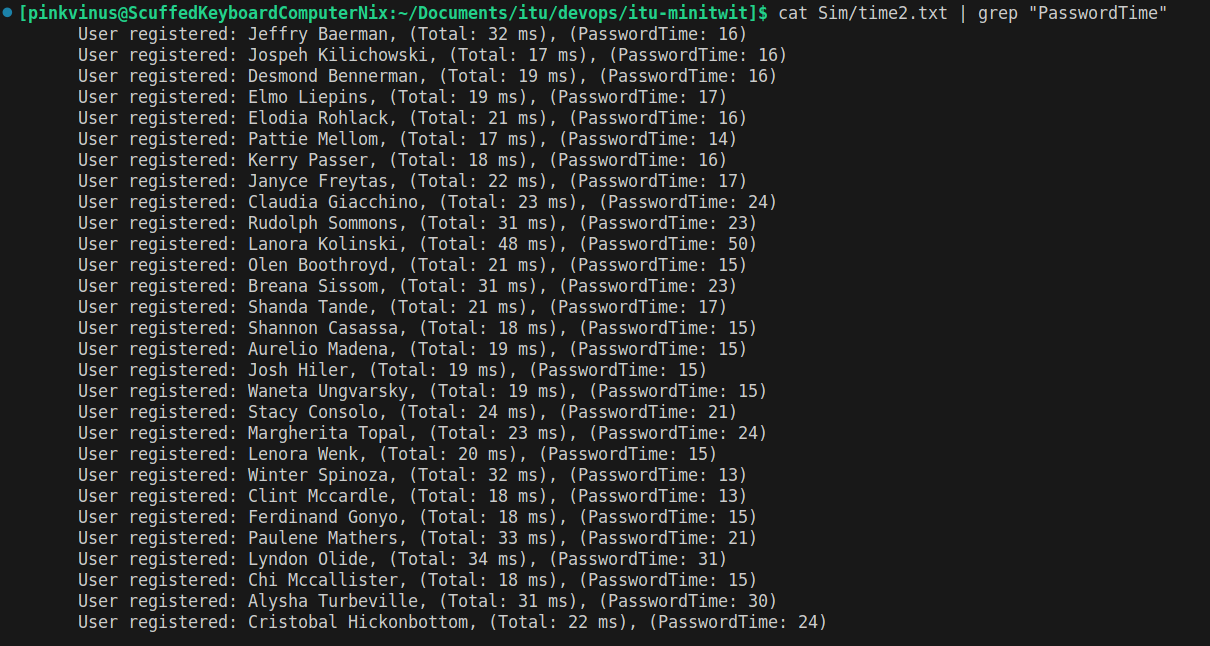
\includegraphics[width=0.7\linewidth]{password.png}
\caption{Results from calling the register endpoint with reduce number of iterations used in hashing}
\end{figure}

Changing the hashing algorithm to SHA512 and changing the number of iterations from 600000 to 210000 as recommended for this algorithm we yields a greater variance in response time, meaning that the fastest responses are faster, and the slowest responses are bout as slow as before. However, due to the fact that we need to be able to hash our already stored passwords, we will have to create a switch in the code, s.t. we would be able to introduce this new password hashing algorithm.

\subsection{Week 9 - 05/04/24}
\label{log:week9}

Tasks: Add scaling to the project, migrate database. Add pre-commit to
devcontainer.

Steps taken:

\subsubsection{Adding pre-commit to devcontainer}
\label{log:adding-pre-commit-to-devcontainer}

This is a task from last week that we didn't manage to finish, as it turned out to be more complicated than we first thought. It has been solved by creating a dockerfile in the devcontainer that install first .net sdk 8, python, hadolint and pre-commit.

Problems i ran into:

\begin{itemize}
    \item I need both sdk 7 and 8, because 7 are used for developing our application since they run in dotnet 7. However, pre-commit uses .net 8 to call the .net formatter. For that reason we need to install sdk 8 in the devcontainer. We tried to use the .net install script but it installed the sdk in a wrong location, so then we used the \texttt{-\/-install-dir} flag to specify the location to install the SDK but for some reason that didn't work either. So we instead installed it at another location and copied the files to the existing installation of dotnet. The script looks like the following:

    \begin{minted}{bash}
        #!/bin/bash

        wget https://dot.net/v1/dotnet-install.sh -O dotnet-install.sh
        chmod +x ./dotnet-install.sh
        ./dotnet-install.sh --version latest --install-dir "/usr/share/dotnet-new"

        sudo cp -u -r /usr/share/dotnet-new/* /usr/share/dotnet/
    \end{minted}

    \item I could tell that my team members couldn't use the devcontainer because they have another cpu, so i found a command that could fix this. The command \texttt{dpkg\ -\/-print-architecture} finds the correct cpu architecture such that the image can run on different systems.
    \begin{minted}{bash}
    hadourl="https://github.com/hadolint/hadolint/releases/download/v2.10.0/hadolint-Linux-$(dpkg --print-architecture)"
    wget -q -O /bin/hadolint $hadourl
    \end{minted}

    \item I didn't have the permission to use hadolint, so i gave the permission in the image with the following command:
    \begin{minted}{bash}
        chmod +x /bin/hadolint
    \end{minted}
\end{itemize}

\subsubsection{Adding scaling to the project}
\label{log:adding-scaling-to-the-project}

\begin{itemize}
    \item Useful resources
    \begin{itemize}
        \item \url{https://docs.ansible.com/ansible/latest/collections/community/docker/docker_swarm_module.html}
        \item \url{https://labouardy.com/setup-docker-swarm-on-aws-using-ansible-terraform/}
        \item \url{https://docs.docker.com/engine/swarm/swarm-tutorial/create-swarm/}
        \item \url{https://www.digitalocean.com/community/tutorials/how-to-create-a-cluster-of-docker-containers-with-docker-swarm-and-digitalocean-on-ubuntu-16-04}
        \item \url{https://www.pulumi.com/registry/packages/digitalocean/api-docs/droplet/}
    \end{itemize}

    How to setup Docker swarm with ansible:

    \begin{itemize}
        \item \href{https://www.youtube.com/watch?v=xZx9XoBnAUI}{Part 1}
        \item \href{https://www.youtube.com/watch?v=qVGO5_bKmpE\&list=PLWZKNB9waqIXEL-NIapWwIADPtkspe9vk\&index=47\&t=201s}{Part 2}
    \end{itemize}
\end{itemize}

We created a new server in the program
\begin{minted}{bash}
$ apt install docker.io
# the ip address here is the private ip for the manager server. (found on digital ocean)
$ docker swarm init --advertise-addr  192.168.1.6
Swarm initialized: current node (qvekvmy3xdpftrheics2kt05v) is now a manager.

To add a worker to this swarm, run the following command:
    docker swarm join --token SWMTKN-1-5bsq5avkideo5oqx6n4b5oth1nhqyg96msjp2igiome125afai-8xk1y3dmymf75zgcia1yrpj2c 192.168.1.6:2377

To add a manager to this swarm, run 'docker swarm join-token manager' and follow the instructions.
\end{minted}

Now we have a swarm manager and a single worker in the swarm

We have found that the lack of documentation has made it very difficult to start working with this task.

\subsubsection{Adding update strategy}
\label{log:adding-update-strategy}

We followed the tutorial linked to us in the lecture slides: \url{https://docs.docker.com/engine/swarm/swarm-tutorial/rolling-update/}

Here we quickly realized that in order to implement an update strategy, we would need a deployed service, which was a part of the `adding scaling to the project' task. We therefore decided to leave this task until the deployment had been implemented and instead fixed the issue about adding UI test for the date formation.

\subsubsection{Migrating Database}
\label{log:migrating-database}

This is the second try, essentially, in migrating the database. We have now noticed a nice and useful guide on how to do it created by \href{https://docs.digitalocean.com/products/databases/postgresql/how-to/import-databases/}{DigitalOcean}.

So the first thing we do is to test it out. So we run our Pulumi workflow to setup our test environment. We then create some scripts to push the dump file that Andreas has of last weeks database to the test server by saying:
\begin{minted}{bash}
    scp dump.sql devops-test:/minitwit/dump.sql
    ssh devops-test

    docker cp /minitwit/dump.sql database:/db-setup/dump.sql

    docker exec database /bin/bash -c "psql -U minitwit-sa minitwit < /db-setup/dump.sql"
\end{minted}

Now that the database has data, we begin using the guide from digitalocean. The setup current is the application server called \texttt{minitwit-test-web-02} and a managed database cluster with a database called \texttt{minitwit}.

According to the guide, we can create the following script:

\begin{minted}{bash}
    #!/bin/bash

    # First we need to run pg_dump for the old database server and save the dump file
    echo "Fetch Database dump from source database"
    pg_dump -h 164.92.253.253 -U minitwit-sa -p 5432 -Fc minitwit > ./minitwit-dump.pgsql

    # Secondly we need to run pg_restore on the new database with the dump file that we have just saved
    echo "Restoring database on target database"
    pg_restore -d <Connection uri string from DO> --jobs 4 ./minitwit-dump.pgsql
\end{minted}

We noticed that if we had to run this on our local laptop then we had to allow the app server to have connections from the public on port \texttt{5432} so we ran the following command on the app server:
\begin{minted}{bash}
    ssh devops-test
    ufw allow in on eth0 to any port 5432
\end{minted}

Another thing is that we had to create a file called \texttt{\textasciitilde{}/.pgpass} . Notice the squiqqly line. According to the postgres documentation it needs to be placed in there. We then add the following content in order to authenticate to the source database:
\begin{minted}{bash}
    164.92.253.253:5432:minitwit:minitwit-sa:<Password of the db user>
\end{minted}

Running the above resulted in an error saying that the \texttt{minitwit-sa} user does not exist. So we create that user in the DigitalOcean UI.

Now that we try to run it again, it fails with the following error:
\begin{minted}{sql}
pg_restore: error: could not execute query: ERROR:  relation "follower" already exists
Command was: CREATE TABLE public.follower (
    who_id integer NOT NULL,
    whom_id integer NOT NULL
);


pg_restore: error: could not execute query: ERROR:  permission denied for schema public
Command was: ALTER TABLE public.follower OWNER TO "minitwit-sa";

pg_restore: error: could not execute query: ERROR:  relation "latest" already exists
Command was: CREATE TABLE public.latest (
    id integer NOT NULL,
    command_id integer NOT NULL
);
\end{minted}

Looking at this could mean that we should refresh that database. So we delete the database and add it again. We then run our script again, and it now fails with the permission denied.

Reading the documentation provided by docker they specify that in some situations you should run the commands with \texttt{—no-owner} when doing \texttt{pg\_restore}. This will not set the owner of the tables. Trying to run the script again removes the permission errors. However, we now encounter the following error:

\begin{minted}{bash}
    pg_restore: error: a worker process died unexpectedly
\end{minted}
By searching through the internet we see one at stackoverflow with a similar \href{https://dba.stackexchange.com/questions/257398/pg-restore-with-jobs-flag-results-in-pg-restore-error-a-worker-process-di}{issue}. We look at the version of postgres installed on our local laptop. But ours is \texttt{16.2} according to the \texttt{pg\_dump\ -\/-version} output. So we did the second option of removing the \texttt{-\/-jobs\ 4} flag. We run it again. And it works!!!

We try to login to the server via pgadmin4 in context of the \texttt{minitwit-sa} which was not the user who created the tables and inserted the data. By doing some select statements on the tables we could see that \texttt{minitwit-sa} does not have access. We give the \texttt{minitwit-sa} access to all tables in the public schema by executing the following query as \texttt{doadmin}:

\begin{minted}{sql}
    GRANT SELECT, UPDATE, INSERT, DELETE ON ALL TABLES IN SCHEMA public TO "minitwit-sa";
\end{minted}

This seems to work! Now the \texttt{minitwit-sa} can select the tables.

After trying to insert and delete entries with the \texttt{minitwit-sa} we saw that it does not have permission to lookup sequences to provide the next id for a user or anything else. So we execute the following command to fix this(as \texttt{doadmin} on the minitwit database):

\begin{minted}{sql}
    GRANT USAGE, SELECT ON ALL SEQUENCES IN SCHEMA public TO "minitwit-sa";
\end{minted}

The final script can be seen at \url{https://github.com/devops2024-group-e/itu-minitwit/commit/fd57686dedf9ebc366f628f52a010f662c1373a5}

\subsubsection{Performing the migration}
\label{log:performing-the-migration}

This is a TODO.

\subsubsection{Save grafana dashboards and datasource files in repo}
\label{log:save-grafana-dashboards-and-datasource-files-in-repo}

So since we are going to move our digital ocean account due to the money expiring, then it will have to move the board. This step here is going to be a simple one. We will have the files that is going to keep the layout. However, the solution will not provide automation to change the endpoints of the datasource. But with this setup it should be easy to change a url and then push it again to see the live dashboards with data.

First we found the following \href{https://github.com/SebastianTorralba/Self-Provisioned-Grafana}{site} that shows how to use the Grafana provisioning feature. So we started by testing it out on a non-production environment. Since we already have a test monitor server, we are going to use that.

We create the same file structure and add the volume paths as it is shown in his Dockerfile.

We then export our existing dashboards to json files and save it in the \texttt{grafana/dashboard} directory.

After that we declare our datasource files. We can extract them as json by doing the following:

\begin{minted}{bash}
    mkdir -p data_sources && \
        curl -s "http://<ip of monitoring server>/api/datasources"  -u admin:admin | \
        jq -c -M '.[]' | split -l 1 - data_sources/
\end{minted}

We then copy them to the \texttt{provisioning/datasources} directory and change them to yaml.

Now on the test server we run \texttt{docker\ compose\ up\ -d} and check that it works. Both the datasources and dashboards is shown.

Now we copy the structure of the directory from the test server to the repo by using \texttt{scp} :

\begin{minted}{bash}
    scp -r devops-test-mon:/minitwit-monitoring/grafana .infrastructure/monitor-server/grafana
\end{minted}

By adding it to the above directory then Ansible should copy those files to the server and use it to start the grafana container.

\subsection{Continuation of fixing the slow response time of the register endpoint}
\label{log:continuation-of-fixing-the-slow-response-time-of-the-register-endpoint}

We had to implement a switch between the former and the current hashing algorithm in order for the \texttt{CheckPasswordHash} method to work with both old and new users in the system. To solve this issue, we made the following chances to /MinitwitSimulatorAPI/Utils/PasswordHash.cs:

\begin{minted}{csharp}
    public static string Hash(string value)
    {
        var salt = RandomNumberGenerator.GetBytes(16);
        return GeneratePasswordHash(value, salt, "SHA512");
    }
\end{minted}

Here we added the string \texttt{“SHA512”} to the values being returned to help us with the switch in the next method.

\begin{minted}{csharp}
    private static string GeneratePasswordHash(string password, byte[] salt, string algorithm)
    {
        string hashedResult;
        string result;
        switch (algorithm)
        {
            case "SHA512":
                hashedResult = Convert.ToHexString(KeyDerivation.Pbkdf2(
                    password: password,
                    salt: salt,
                    prf: KeyDerivationPrf.HMACSHA512,
                    iterationCount: 21000,
                    numBytesRequested: 32));
                result = $"SHA512${Convert.ToHexString(salt)}${hashedResult}";
                break;
            default:
                hashedResult = Convert.ToHexString(KeyDerivation.Pbkdf2(
                    password: password,
                    salt: salt,
                    prf: KeyDerivationPrf.HMACSHA256,
                    iterationCount: 600000,
                    numBytesRequested: 32));
                result = $"{Convert.ToHexString(salt)}${hashedResult}";
                break;
        }
        return result;
    }
\end{minted}

We now check in the switch statement whether we got the \texttt{“SHA512”} string from the \texttt{Hash} method.

If we do, then we run the current hash algorithm, where we have lowered the number of iterations to 21000, which is a tenth of the recommend number from OWASP. We also add ``SHA512'' to the beginning of the password, which is needed in the \texttt{CheckPasswordHash} method in order to differentiate between the two versions of the algorithm.

If we didn't get the \texttt{“SHA512”} string, then we run the former hash algorithm, which hasn't been changed and still has the recommended number of iterations.

\begin{minted}{csharp}
    public static bool CheckPasswordHash(string password, string hashedPassword)
    {
        var passwordParts = hashedPassword.Split('$');

        string pp;

        switch (passwordParts[0])
        {
            case "SHA512":
                pp = GeneratePasswordHash(password, Convert.FromHexString(passwordParts[1]), "SHA512");
                break;
            default:
                pp = GeneratePasswordHash(password, Convert.FromHexString(passwordParts[0]), "SHA256");
                break;
        }
        return pp == hashedPassword;
    }
\end{minted}

We check in the switch statement whether the password include the \texttt{“SHA512”} string at the start in order to determine whether to run the current or the former hashing algorithm.

\subsection{Week 10 - 12/04/24}
\label{log:week10}

Tasks: Switch Digital Ocean account, continue adding scaling to the project, add documentation and mapping of the system

Steps taken:

\subsection{Finalization of fixing the slow response time of the register endpoint}
\label{log:finalization-of-fixing-the-slow-response-time-of-the-register-endpoint}

To complete the task of fixing the slow response time in the register endpoint, we needed to create tests to make sure that the hashing algorithm worked as we had intended.

These tests are located in Minitwit.Simulator.Api.Tests/Controllers/RegisterControllerTests.cs

We ran Helge's minitwit simulator with both the former and the current version of the hashing algorithm in order to get hashed passwords that matched with users in the database. We then selected 3 different users with both versions of their hashed password in order to test that the correct usage of the passwords would return true and messing with their passwords would return false.

We had some trouble getting the PR for this issue accepted on GitHub due to pre-commit in the testing workflow raising an exception we couldn't replicate locally, but this was fixed by adding dotnet 8 to the pre-commit step.

\subsection{Mapping the system}
\label{log:mapping-the-system}

To map the system, we looked through our decision log to get an overview over the different tools we have introduced throughout the project. We also looked at Digital Ocean to get a sense of the servers and through our GitHub repository in order to recall details about how we set up certain features. We decided to do an abstract overview of the system, as this was meant to help us keep track of how everything is connected and work with each other.

We added very short descriptions to each element in the diagram as separate text in order to give a quick overview. The decision log is meant for more lengthy paragraphs justifying our decisions, whereas this is meant for making sense of the system as a single unit.

\subsection{Refactor FollowerController in SimulatorAPI}
\label{log:refactor-followercontroller-in-simulatorapi}

In order to get cleaner code we have refactored one of the methods in the FollowerController to receive follow/unfollow information via a method parameter instead of using a streamreader and other weird stuff.

\subsection{Week 11 - 19/04/24}
\label{log:week11}

Tasks: Add one more frontend replica. Make security assessment. Handled
a hacking attack!!

Steps taken:

\subsubsection{Add one more frontend replica:}
\label{log:add-one-more-frontend-replica}

\begin{itemize}
    \item In order for this to work we need the frontend to make use of sessions so that it still remembers who is logged in based on the id. Therefore we have added a session table in the database.
    \item We have added one more replica of the frontend such that there is now two of them.
\end{itemize}

We wanted to add one more frontend replica and that could be seen as a simple task, it sounds like we just need to add 2 instead of 1 in \texttt{.infrastructure/servers/swm-server/docker-compose.yaml}. The problem is that we use sessions for keeping track of the current users user\_id. This session is in the memory of the frontend instance which means that the session will be lost when switching replicas. To solve this we started looking in to these two links that explained how to write code to be able to handle distributed sessions.

\url{https://learn.microsoft.com/en-us/aspnet/core/fundamentals/app-state?view=aspnetcore-8.0}

\url{https://www.nuget.org/packages/Community.Microsoft.Extensions.Caching.PostgreSql}

We started to add code for handling distributed sessions:

We added this package PostgreSQL in \texttt{Minitwit/Minitwit.csproj}:

\begin{minted}{xml}
    <PackageReference Include="Community.Microsoft.Extensions.Caching.PostgreSql" Version="4.0.4" />
\end{minted}

We added sessions settings in \texttt{Minitwit/project.cs}:

\begin{minted}{csharp}
    builder.Services.AddDistributedPostgreSqlCache(setup =>
    {
        setup.ConnectionString = builder.Configuration.GetConnectionString("MinitwitDatabase");
        setup.SchemaName = "public";
        setup.TableName = "session";
        setup.DisableRemoveExpired = false;
        setup.CreateInfrastructure = false;
        setup.ExpiredItemsDeletionInterval = TimeSpan.FromMinutes(15);
    });

    builder.Services.AddSession(options =>
    {
        options.IdleTimeout = TimeSpan.FromMinutes(5);
        options.Cookie.HttpOnly = true;
        options.Cookie.IsEssential = true;
    });
\end{minted}

and added a session table in \texttt{schema.sql}:
\begin{minted}{sql}
    create table if not exists "session"
    (
        "Id" text COLLATE pg_catalog."default" NOT NULL,
        "Value" bytea,
        "ExpiresAtTime" timestamp with time zone,
        "SlidingExpirationInSeconds" double precision,
        "AbsoluteExpiration" timestamp with time zone,
        CONSTRAINT "DistCache_pkey" PRIMARY KEY ("Id")
    );
\end{minted}

We then pulled it in to main without any errors or problem from the testing. When we went to the website and tried to log in, now with two replicas, we noticed that when we did log in we could see the text ``You're now logged in'' but we still were not properly logged in and couldn't do any of the task we usually can. We could therefore see that the distributed sessions isn't working as they should.

First we checked if the database was correctly connected and could see that it wasn't. So we fixed a proper connection but still had the same problems.

We also tried to set upp the distributed sessions with redis as image in \texttt{.devcontainer/docker-compose.yaml}

\begin{minted}{yaml}
        - main
    environment:
      - Minitwit_ConnectionStrings__MinitwitDatabase=Host=minitwit-dev-database;Port=5432;Username=minitwit-sa;Password=123;Database=minitwit
      - Minitwit_ConnectionStrings__Redis=minitwit-cache:6379

  minitwit-db:
    build:
@@ -27,3 +28,11 @@ services:
      - main
    ports:
      - '5432:5432'

  cache:
    image: redis:7.2.4
    container_name: minitwit-cache
    networks:
      - main
    ports:
      - '6379:6379'
\end{minted}

And added arguments for the secrets in \texttt{.github/workflows/Provision-and-Deploy.yaml} file:

\begin{minted}{bash}
    build-args: |
            DB_CONN=${{ secrets.DB_CONNECTION }}
            REDIS_CONN=${{ secrets.REDIS_CONNECTION }}
\end{minted}

and testing if it's the image is deployed in.\texttt{github/workflows/Testing.yaml}:

\begin{minted}{yaml}
     - name: Set up redis cache
       run: docker compose -f docker-compose.yaml up cache -d
\end{minted}

Specified it in \texttt{.infrastructure/servers/swm-server/docker-compose.yaml:}

\begin{minted}{yaml}
      cache:
      image: redis:7.2.4
      networks:
        - main
      ports:
        - '6379:6379'
\end{minted}

In \texttt{Dockerfile.frontend} we added:

\begin{minted}{text}
    ARG REDIS_CONN=""
\end{minted}

and:

\begin{minted}{bash}
    ENV Minitwit_ConnectionStrings__MinitwitDatabase=${REDIS_CONN}
\end{minted}

In \texttt{Minitwit/Minitwit.csproj} we added two packages:

\begin{minted}{xml}
    <PackageReference Include="Microsoft.Extensions.Caching.StackExchangeRedis"
        Version="7.0.18" />
\end{minted}

\begin{minted}{xml}
    <PackageReference Include="StackExchange.Redis"
        Version="2.7.33" />
\end{minted}

And in the \texttt{Minitwit/Program.cs} we changed up the code for how to handle the cached sessions:

\begin{minted}{csharp}
    builder.Services.AddStackExchangeRedisCache(options =>
    {
	    options.Configuration = builder.Configuration.GetConnectionString("Redis");
    options.InstanceName = "minitwit_";
    });

    builder.Services.AddSession(options =>
    {
        options.IdleTimeout = TimeSpan.FromMinutes(5);
        options.Cookie.HttpOnly = true;
        options.Cookie.IsEssential = true;
    });
\end{minted}

In the \texttt{Minitwit/appsettings.Development.json} file we specified the connection string and the port:

\begin{minted}{json}
    "ConnectionStrings": {
        "MinitwitDatabase": "Host=127.0.0.1;Port=5432;Username=minitwit-sa;Password=123;Database=minitwit"
        "MinitwitDatabase": "Host=127.0.0.1;Port=5432;Username=minitwit-sa;Password=123;Database=minitwit",
        "Redis": "localhost:6379"
    }
\end{minted}

and lastly we added this code to \texttt{docker-compose.yaml}:

\begin{minted}{yaml}
  cache:
    image: redis:7.2.4
    container_name: minitwit-cache
    networks:
      - main
    ports:
      - '6379:6379'
\end{minted}

After this we pulled to main again and tried to log in to Minitwit again and could then see that it still didn't work and that we had the same problem as before, that we got the logged in message but still wasn't properly logged in. After all the time we put on trying to make this work we decided that the problem itself isn't so essential that we should put anymore time on it. We therefore revoked all of the changes we previously made and went back to having one replica for the frontend instead.

\subsubsection{Make security assessment:}
\label{log:make-security-assessment}

The security assessment can be seen in a separate document.

\subsubsection{Got hacked and handled it:}
\label{log:got-hacked-and-handled-it}

We got hacked as described in another document. We deleted our docker
swarm servers with Pulumi to get rid of it.

\subsection{Week 12 - 26/04/24}
\label{week12}

Tasks: Harden the system based on our security assessment from last week. Prepare diagrams of the system.

Steps taken:

\subsubsection{Harden the system based on our security assessment from last week:}
\label{log:harden-the-system-based-on-our-security-assessment-from-last-week}

\begin{itemize}
\item Close ports:

    \begin{itemize}
        \item We started by using \emph{Kali Linux} to run \textbf{nmap}, which told us of the following open ports in our system:
        \begin{figure}[H]
        \centering
        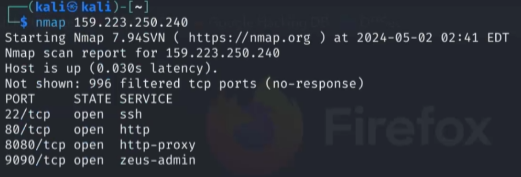
\includegraphics[width=0.7\linewidth]{port-scan.png}
        \caption{Results from running \texttt{nmap}}
        \end{figure}
        The 22/tcp is for \emph{ssh}, the 80/tcp and 8080/tcp are for \emph{http} and the 9090/tcp is for \emph{Prometheus}, where the latter doesn't require an open port. To fix this, we instead exposed the port to a private network via the interface eth1 and denied access via eth0.

        When we went into the shell of the server, we could see that the firewall was working as expected, but we were still being told by nmap that port 9090 was open. After trying to remove all access to port 9090 and not seeing any changes in Kali Linux, we went back to the solution described above and left if for Friday to investigate further.

        \item We then ran \textbf{OWASP zap} to scan our website for vulnerabilities in regards to the ports. This showed us some warnings about not being fully protected from injection attacks or attacks made with the header, but none about the ports, so we didn't make any actions from this.
        \item Lastly, we wanted to upgrade the system from HTTP to \textbf{HTTPS}, as the former is not secure and this would likely solve some of our security issues. To do this, we tried to follow the guide made by Mircea from the 11th lecture:

        \begin{itemize}
            \item First attempt

            \begin{enumerate}
                \item Create a domain -> We bought the domain \href{http://grlpwrtwit.dk}{grlpwrtwit.dk} on simply.com
                \item Set the name servers -> This is where we ran into a lot of issues. Whenever we tried to change the name servers on simply.com, we got an error message saying to control what we wrote. After doing some digging, we found a post that said \href{http://Punktum.dk}{Punktum.dk} was where we had to go to change the name servers due to our domain ending in .dk. Again, we tried to follow the online tutorials, but we didn't have access to the correct link as shown in the guides.
                Creating tickets and trying to reach out to the support on      \href{http://simply.com}{simply.com} didn't help either.
            \end{enumerate}
            \item Second attempt

            \begin{enumerate}
                \item Create a domain -> We bought the domain grlpwrtwit.se on Loopia.se
                \item Set the name servers -> We here had to first disable DNSSEC and then we were able to change the name servers to \href{http://ns1.digitalocean.com}{ns1.digitalocean.com} and \href{http://ns2.digitalocean.com}{ns2.digitalocean.com} as told by the guides.
            \end{enumerate}
        \end{itemize}
    \end{itemize}
    \item Prevent injection via logging:

    \begin{itemize}
        \item The user inputs have been sanitised in order to prevent injection attacks. Before the user input was put directly into logging. We have now replaced newlines \texttt{\textbackslash{n}} and carriage returns '\r' with '\_'.
    \end{itemize}
    \item Update dependencies in pipeline:

    \begin{itemize}
        \item Enabled security checks and package updates by dependabot in github repo security settings
        \item Added \texttt{dependabot.yml} config file to workflow, which checks Github Actions and NuGet packages for outdated dependencies.
        \item Dependabot automatically adds PRs to the project for outdated packages
    \end{itemize}
\end{itemize}
